\section{Projektmanagement}

\subsection{Projektübersicht}
Das Hauptziel dieser Studienarbeit ist die Installation von DNA-Center und Integration vom bestehenden Labor-Netzwerk.

\subsubsection{Ziele der Projektes}
Da Software-Defined Access Neuland im Campus Bereich ist, wollen wir die SD-Access Lösung vom Hersteller Cisco ausarbeiten. Dazu gehören folgende Ziele:

\begin{itemize}
	\item Installation von DNA-Center und Integration vom bestehenden Campus Labor-Netzwerk.
	\item Definieren von Benutzer- und Geräteprofilen, um basierend auf Geschäftsanforderungen die Zugriffsrechte und Netzwerksegmentierung zu veralten und so das Netzwerk sicher zu halten.
	\item Verwendung von Erkenntnissen von DNA Analytics and Assurance für eine proaktive Überwachung, Fehlerbehebung und Optimierung des Netzwerks.
	\item Integration vom bestehenden IP Address Management Tool im DNA Center
	\item Durch APIs, Erstellung von wöchentlichen Reports über den Campus Netzwerk Status in einem E-Mail und einer Slack Message. 
\end{itemize}

\subsection{Projektorganisation}
Diese Studienarbeit wird von drei Personen umgesetzt und durch zwei Betreuer überwacht.

\subsubsection{Organisationsstruktur}
\begin{figure}[H]
	\centering
	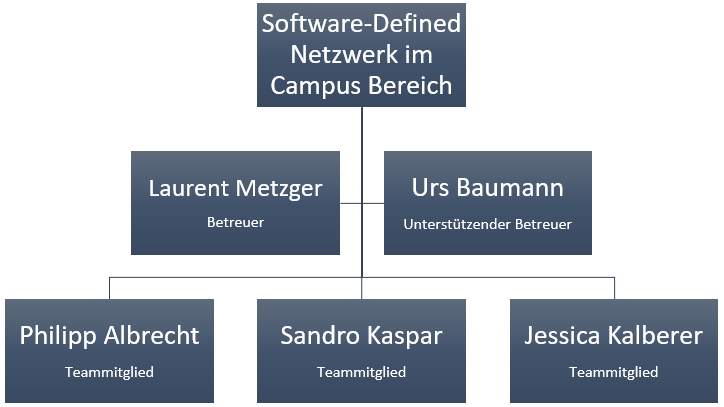
\includegraphics[height=5cm]{img/Organisationsstruktur.png}
	\caption{Organisationsstruktur}
	\label{fig:Organisationsstruktur}
\end{figure}

\subsection{Management Abläufe}
\subsection{Kostenvoranschlag}
Für die Umsetzung der Studienarbeit stehen insgesamt 15 Wochen und pro Person 240 Stunden zur Verfügung. In einer Woche liegt das Arbeitspensum von 16 Stunden pro Person vor. Das Projekt startet am 19. Februar 2018 und endet am 1. Juni 2018.

\subsubsection{Zeitliche Planung}
Die zeitliche Planung erfolgte in Gant und die Verwaltung der Arbeitspakete auf Waffle.io. Die Planung wird während dem Projekt laufend aktualisiert und angepasst. Die Zeiterfassung erfolgt während der Arbeitsausführung mittels Tracking in Toggle.

\begin{figure}[H]
	\centering
	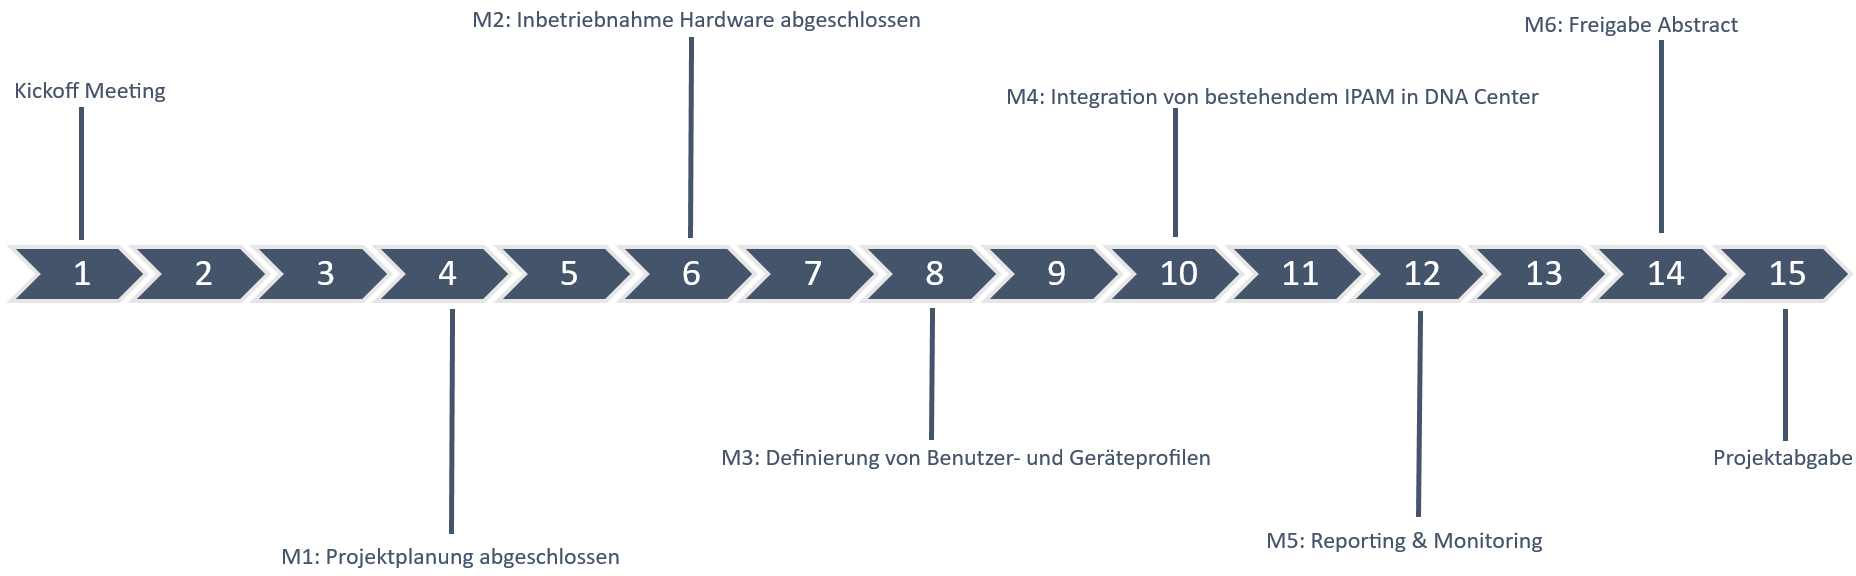
\includegraphics[height=5cm]{img/ZeitlichePlanung.png}
	\caption{Projektplanung}
	\label{fig:Projektplanung}
\end{figure} 

\subsection{Infrastruktur}

\begin{figure}[H]
	\centering
	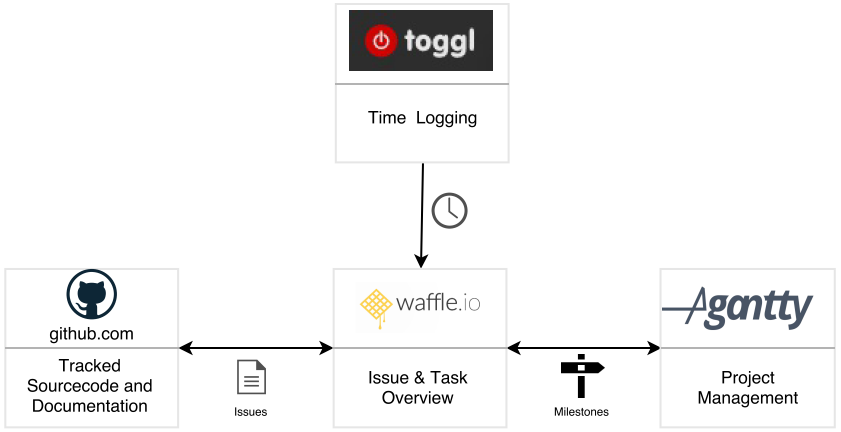
\includegraphics[height=6cm]{img/InterneOrganisationsstruktur.png}
	\caption{Interne Organisationsstruktur}
	\label{fig:Interne Organisationsstruktur}
\end{figure} 

\subsection{Risiko Management}

\subsubsection{Umgang mit Risiken}

Risiken lassen sich leider nicht immer vermeiden. Aus diesem Grund sind nachfolgend mögliche Risiken aufgeführt. Des Weiteren wurden vorbeugende Massnahmen definiert um die Eintretenswahrscheinlichkeit von Risiken mit schwerwiegenden Konsequenzen zu reduzieren. Für den Fall, dass ein Risiko dennoch eintreten sollte, sind entsprechende Massnahmen definiert um den Schaden möglichst gering zu halten.
Sollten sich während dem Projekt neue potenzielle Risiken zeigen, wird dieses Dokument laufend aktualisiert.

\begin{landscape}

\subsubsection{Risiken}
\newcommand*\rot{\rotatebox{90}}
\begin{longtable}{|m{0.5cm}|m{3cm}|m{5cm}|m{0.75cm}|m{0.75cm}|m{0.75cm}|m{5cm}|m{5cm}|} 
	\hline
	\rot{Nummer} & \rot{Titel} & \rot{Beschreibung} & \rot{\shortstack[l]{maximaler\\Schaden [h]}} & \rot{\shortstack[l]{Eintritts-\\wahrscheinlichkeit}} & \rot{\shortstack[l]{Gewichteter\\Schaden [h]}} & \rot{Vorbeugung} & \rot{\shortstack[l]{Verhalten beim\\Eintreten}} \\
	\hline\hline
	1 & Ausfall eines Teammiglieds & Ausfall auf Grund unvorhergesehener Erreignisse wie Krankheit, Unfall etc. & 40 & 15\% & 6 & Reserven einplanen, Kommunikation sicherstellen, sodass der Rest Aufgaben übernehmen kann & Tasks des ausgefallen Mitglieds möglichst auf den Rest des Teams aufteilen. \\ 
	\hline
	2 & Hardwareausfall DNA-Center & DNA-Center Appliance fällt durch Hardwaredefekt aus & 30 & 5\% & 1.5 & keine Verbeugenden Massnahmen möglich & Austausch im Rahmen der Garantie veranlassen \\
	\hline
	3 & Fehlendes Know How & Da viele der Themen neu sind, kann entsprechendes Wissen fehlen & 40 & 20\% & 8 & Zeit einplanen um sich in neue Themen einzuarbeiten & Fehlendes Wissen sobald wie möglich aneignen. Bei Bedarf Rat der Betreuer einholen \\
	\hline
	4 & Konflikte oder Missverständnisse im Team & Das Team ist sich bezüglich wichtigen Entscheidungen uneinig & 25 & 15\% & 3.75 & Entscheidungen stets mit Begründung dokumentieren & Kann auch mit Hilfe der Doku keine Einigung gefunden werden, fachnlichen Rat des Betreuers einholen \\
	\hline
	5 & Missverständnisse im Team & Im Team herscht Uneinigkeit über bereits getroffene Entscheidungen & 20 & 20\% & 4 & Protokolle führen und Entscheidungen klar dokumentieren & Protokolle und Dokumentationen beiziehen \\
	\hline
	6 & Ausfall Server / Netzwerkinfrastruktur & Ausfall der von der HSR zur Verfügung gestellten Infrastrukturkomponenten & 30 & 10\% & 3 & Keine Vorbeugenden Massnahmen möglich & Sobald die Infrastruktur wieder verfügbar ist, Systeme wieder in Betrieb nehmen \\
	\hline
	7 & Lieferverzögerung Hardware & Die von Cisco bestellte Hardware kommt später als angekündigt & 30 & 18\% & 5.4 & Keine Vorbeugenden Massnahmen möglich & Projektplanung an neue Gegebenheiten anpassen, notfalls Projektumfang anpassen \\
	\hline
	8 & Zeitaufwände falsch geschätzt & Auf Grund falscher Schätzungen kommt es zu Verzögerungen im Projekt & 30 & 25\% & 7.5 & Laufende Kontrolle des Projektfortschritts um Probleme frühzeitig zu erkennen, Reserven einplanen & Verbleibende Schätzungen korrigieren, Planung anpassen \\
	\hline
	9 & Datenverlust & Verlust von projektbezogenen Daten wie Dokumentationen, Konfigurationen etc. & 40 & 5\% & 2 & Regelmässige und verteilte Backups aller Daten erstellen & Verlorenen Daten aus Backups wiederherstellen, fehlende Daten neu erarbeiten \\
	\hline
\end{longtable}

\end{landscape}

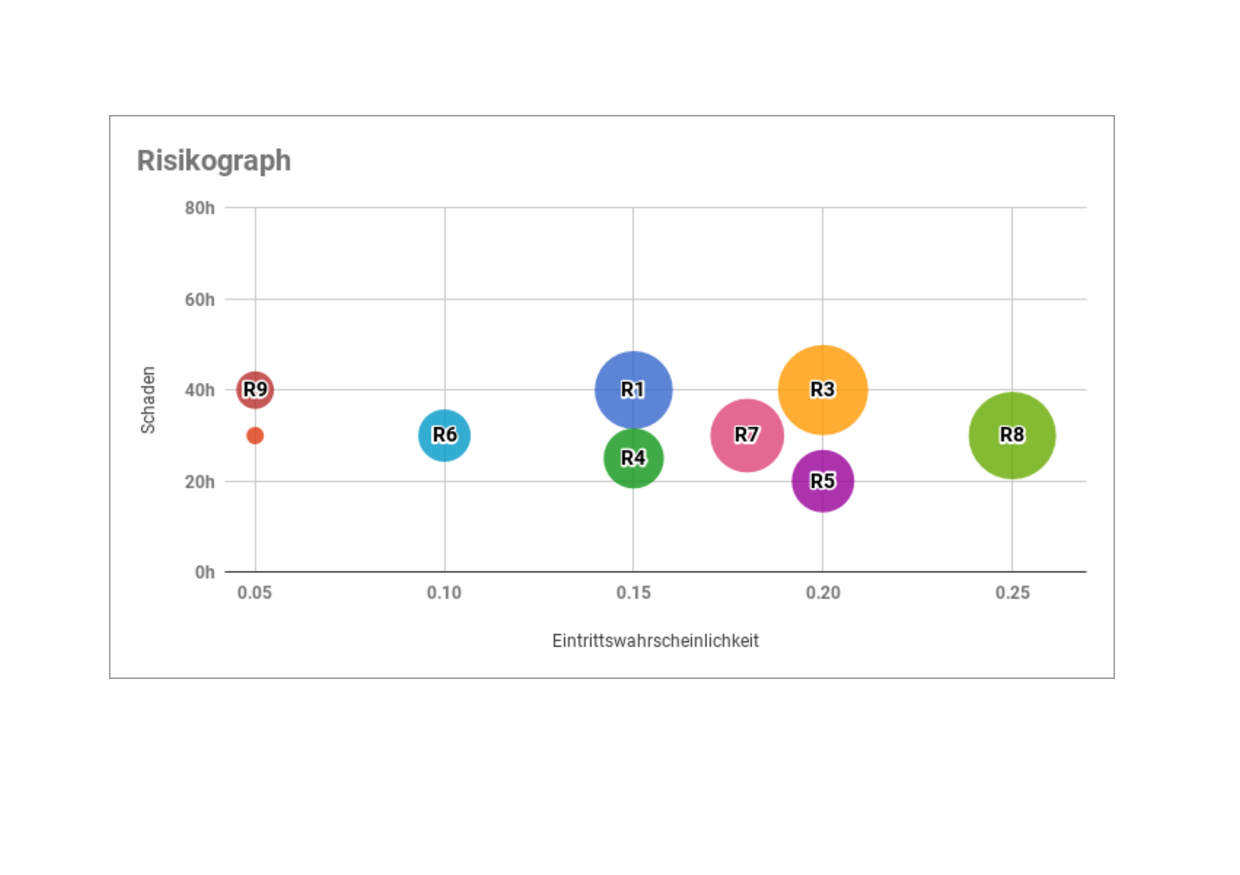
\includepdf{pdfincludes/risikograph}



